\documentclass[a4paper,10pt,ngerman]{scrartcl}
\usepackage{babel}
\usepackage[T1]{fontenc}
\usepackage[utf8x]{inputenc}
\usepackage[a4paper,margin=2.5cm]{geometry}

% Die nächsten drei Felder bitte anpassen:
\newcommand{\Name}{BANDO} % Teamname oder eigenen Namen angeben
% \newcommand{\TeamId}{}
\newcommand{\Aufgabe}{Brainfire: \LaTeX-Dokumentation}

% Kopf- und Fußzeilen
\usepackage{scrlayer-scrpage}
\setkomafont{pageheadfoot}{\textrm}
\ifoot{\Name}
\cfoot{\thepage}
\chead{\Aufgabe}
% \ofoot{Team-ID: \TeamId}

% Für mathematische Befehle und Symbole
\usepackage{amsmath}
\usepackage{amssymb}

% Für Bilder
\usepackage{graphicx}

% Für Algorithmen
\usepackage{algpseudocode}

% Für Quelltext
\usepackage{listings}
\usepackage{color}
\definecolor{mygreen}{rgb}{0,0.6,0}
\definecolor{mygray}{rgb}{0.5,0.5,0.5}
\definecolor{mymauve}{rgb}{0.58,0,0.82}
\lstset{
  keywordstyle=\color{blue},commentstyle=\color{mygreen},
  stringstyle=\color{mymauve},rulecolor=\color{black},
  basicstyle=\footnotesize\ttfamily,numberstyle=\tiny\color{mygray},
  captionpos=b, % sets the caption-position to bottom
  keepspaces=true, % keeps spaces in text
  numbers=left, numbersep=5pt, showspaces=false,showstringspaces=true,
  showtabs=false, stepnumber=2, tabsize=2, title=\lstname
}
\lstdefinelanguage{JavaScript}{ % JavaScript ist als einzige Sprache noch nicht vordefiniert
  keywords={break, case, catch, continue, debugger, default, delete, do, else, finally, for, function, if, in, instanceof, new, return, switch, this, throw, try, typeof, var, void, while, with},
  morecomment=[l]{//},
  morecomment=[s]{/*}{*/},
  morestring=[b]',
  morestring=[b]",
  sensitive=true
}

% Diese beiden Pakete müssen als letztes geladen werden
\usepackage{hyperref} % Anklickbare Links im Dokument
\usepackage{cleveref}

% Daten für die Titelseite
\title{\Aufgabe}
\author{\Name}
\date{\today}



\begin{document}
	
	\maketitle
	\tableofcontents
	
	
	\section{Pathfinder-Generierung}
		
		\subsection{Grundidee}
		
			Betrachte die zwei Punkt S (für "'Start"') und Z (für "'Ziel"') in einem Raum. Da der Raum in seiner Ausbreitung beschränkt ist, existieren von S zu Z - bei gewünschter Platzierung der Steine - auch nur eine endliche Anzahl an denkbarer Lösungspfade. Ein Algorithmus soll all diese Pfade bestimmen, sortieren und speichern. Die für einen Pfad notwendigen Steine sollen ebenfalls gespeichert werden, aber auch die Menge aller Felder, die nicht mit Steinen belegt werden dürfen.
			
			Wann immer ein Raum generiert werden soll, sodass mindestens eine Lösung von S nach Z existiert, so ist es hinreichend einen Pfad der gespeicherten Menge zufällig auszuwählen und die entsprechenden Felder mit Steinen zu belegen bzw. freizuhalten. Mögliche Laufzeit-Probleme sind auf diese Weise auf einen Zeitpunkt vor Beginn des Spiels verschoben worden. Das eigentliche Spiel bedarf auch nicht eines Algorithmus, der die Existenz einer Lösung sicherstellt.\\
			
			tl;dr: Die Eigenschaft, dass mindestens ein Lösungspfad von S nach Z in einem Raum existiert, wird durch eine zuvor untersuchte und langfristig gespeicherte Menge definiert.
		
		\subsection{Umsetzbarkeit}
		
			Um die Idee auf Umsetzbarkeit zu überprüfen, wurde ein Backtracking-Algorithmus geschrieben, der strukturiert alle Lösungspfade von S nach Z in einem beliebig großen Raum bestimmt. Obwohl die Punkte S und Z frei wählbar sind, wurden sie wie im Skript festgelegt: S ist ein Feld unter der links oberen Ecke und Z ist ein Feld über der rechts unteren Ecke.
			
			\begin{figure}[h!]
				\begin{center}
					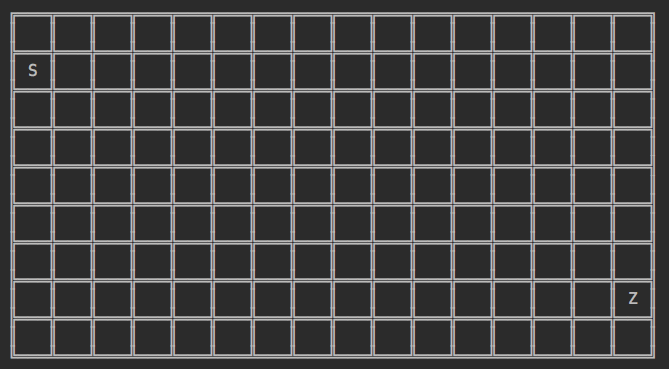
\includegraphics[width=1\textwidth]{SZ.png}
					\caption{Position von S und Z in einem 16 mal 9 Raum}
				\end{center}
			\end{figure}
			\newpage
			
			Der Algorithmus lieferte die Menge aller Lösungspfade und insbesondere auch die Anzahl der Lösungen. Folgende Tabelle hält die Menge aller Lösungen abhängig von der Dimension des Raums fest:
			
			\begin{figure}[h!]
				\begin{center}
					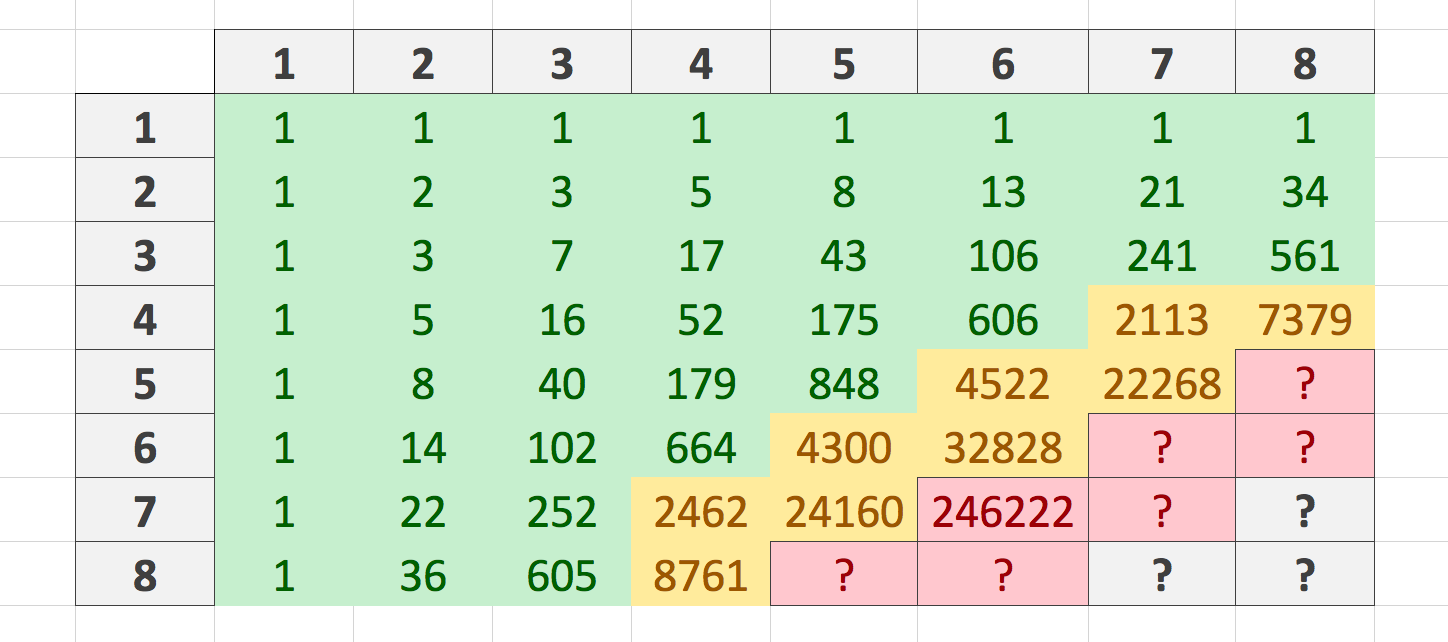
\includegraphics[width=1\textwidth]{Laufzeittabelle.png}
					\caption{Menge aller Lösungen in Abhängigkeit von Breite und Höhe des Raums}
				\end{center}
			\end{figure}
			
			Das Fazit, das aus dieser Betrachtung gezogen werden kann, ist, dass alle Raumgrößen im grauen Bereich der Tabelle nicht denkbar für diesen Generierungsansatz sind. Im besten Fall ist dieser Algorithmus für maximal 7x7 große Räume nutzbar.
		
		\newpage
		\subsection{Beispiel}
		
			\begin{figure}[h!]
				\begin{center}
					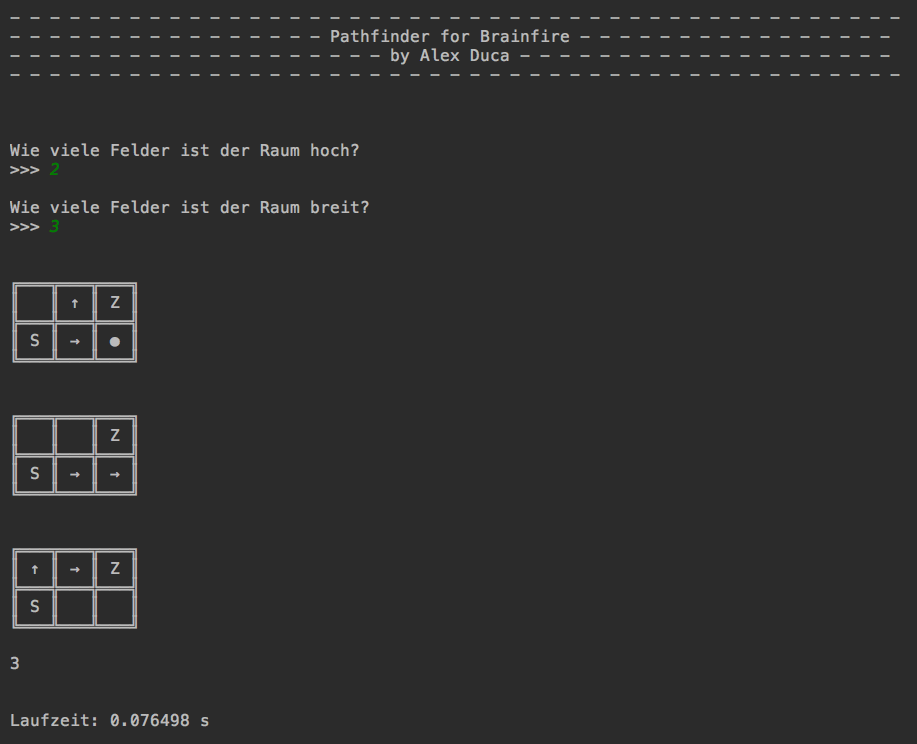
\includegraphics[width=1\textwidth]{2x3Beispiel.png}
					\caption{Menge aller Lösungen in einem 2x3-Raum}
				\end{center}
			\end{figure}
		
		\subsection{Quellcodeausschnitt}
		
		Methode, die das Backtracken in Gang setzt.
		
		\begin{lstlisting}[language=Python]
			alleRaeume = []
			Richtungen = [ (1,0), (0,1), (-1,0), (0,-1) ]
			
			def startBacktracking(Matrix):
			
				# Globale Informationen
				global alleRaeume
				alleRaeume = []
				backupKopieMatrix = deepcopy(Matrix)
				
				# Probiere in alle Richtungen
				for richtung in Richtungen:
				
					neuePos = startPos
					Matrix = deepcopy(backupKopieMatrix)
					
					while True:
					
						altePos = neuePos
						
						# Probiere einen Schritt nach vorne
						neuePos = ( altePos[0] + richtung[0], altePos[1] + richtung[1] )
						
						# Wenn du gegen eine Wand stoesst
						if not inRange(neuePos):
							# Wenn diese Wand nicht gleich am Anfang ist, dann backtracke
							if altePos != startPos:
								backtracking(Matrix, altePos, richtung)
								# Wir sind dann auch fertig fuer die Richtung
								break
						
						# Lege einen Pfeil auf dem Boden in aktuelle Laufrichtung
						Matrix[neuePos[0]][neuePos[1]] = pfeil(richtung)
						
						
						# Versuche einen Stein vor die neue Position zu legen und starte Backtracking
						stein = ( neuePos[0] + richtung[0], neuePos[1] + richtung[1] )
						if inRange(stein):
						
							Matrix[ stein[0] ][ stein[1] ] = "O"
							backtracking(Matrix, neuePos, richtung)
							
							# Nach erfolgreichem Steinelegen, nimm ihn wieder weg und lauf weiter in die Richtung
							Matrix[ stein[0] ][ stein[1] ] = " "
				
				
				for Raum in alleRaeume:
				printMatrixRaum(Raum)
				print(len(alleRaeume))
		\end{lstlisting}
		
		Methode, die beim Backtracking rekursiv aufgerufen wird.
		
		\begin{lstlisting}[language=Python]
			def backtracking(Matrix, eigenePos, letzteRichtung):
			
			# Globale Informationen
			global alleRaeume
			backupKopieMatrix = deepcopy(Matrix)
			
			# Sind wir schon am Ziel?
			if eigenePos == endPos:
				backupKopieMatrix[endPos[0]][endPos[1]] = "Z"
				alleRaeume.append(backupKopieMatrix)
			
			else:
				# lauf nur links oder rechts
				Senkrechten = senkrechte(letzteRichtung)
				for richtung in Senkrechten:
					
					neuePos = eigenePos
					Matrix = deepcopy(backupKopieMatrix)
					
					while True:
					
						altePos = neuePos
						
						# Probiere einen Schritt nach vorne
						neuePos = (altePos[0] + richtung[0], altePos[1] + richtung[1])
						
						# Ist da eine Wand?
						if not inRange(neuePos):
							# Wir koennen hier aufhoeren
							break
						
						# Liegt da ein Stein?
						elif Matrix[ neuePos[0] ][ neuePos[1] ] == "O":
							# Wir koennen hier aufhoeren
							break
						
						# Ist der Boden NICHT mit einem Pfeil markiert?
						elif Matrix[ neuePos[0] ][ neuePos[1] ] == " ":
						
							# Markiere den Boden mit einem Pfeil
							Matrix[neuePos[0]][neuePos[1]] = pfeil(richtung)
							
							# Potentielle Abbiegung gefunden!
							stein = (neuePos[0] + richtung[0], neuePos[1] + richtung[1])
							
							# Ist dort, wo der Stein liegen sollte, schon eine Wand?
							if not inRange(stein):
								# Wenn Ja, dann kann man von der Wand aus abbiegen
								backtracking(Matrix, neuePos, richtung)
							
							# Wenn Nein, liegt dort schon ein Stein?
							elif Matrix[ stein[0] ][ stein[1] ] == "O":
								# Wenn Ja, dann kann man von dem Stein aus abbiegen
								backtracking(Matrix, neuePos, richtung)
							
							# Wenn Nein, ist die Flaeche frei fuer ein Stein?
							elif Matrix[ stein[0] ][ stein[1] ] == " ":
								# Platziere einen Stein und biege ab!
								Matrix[stein[0]][stein[1]] = "O"
								backtracking(Matrix, neuePos, richtung)
								# Und lege ihn danach wieder weg
								Matrix[stein[0]][stein[1]] = " "
		\end{lstlisting}

	
	\newpage
	\section{Gestaltung der Hintergrundmusik}
	
		\subsection{Inspirationsquellen}
		
			Da die Spielmechanik die Fortbewegung auf einer Eisfläche ist, soll Inspiration von Videospielmusikstücken gezogen werden, die ein Kälte-Motiv haben. Im Folgendem findet sich eine solche Auswahl.
			
			\subsubsection{The Legend of Zelda: Ocarina of Time}
			
				"'Ice Cavern"' (\href{https://youtube.com/watch?v=bcXuwXKsqMY}{bit.ly/2L22Kf2}) ist eine Eishöhle, in der Link unter anderem riesige Blöcke über einem Eisboden rutschen lässt, um eine Treppe zu seinem Ziel zu bauen. (\href{https://youtube.com/watch?v=uaGb3PtSPDg}{bit.ly/2LbnzDH})
			
			
			\subsubsection{The Legend of Zelda: Majora's Mask}
			
				"'Snowhead Temple"' (\href{https://youtube.com/watch?v=uxPDVDpbskI}{bit.ly/2Uc8sOl}) ist ein hoher zugefrorener Turm, zu dessen Spitze Link navigieren muss. In der Mitte des Turms findet sich eine Säule, dessen Höhe anpasst werden muss, indem von Goronen-Link vereinzelte Eisschichten aus der Säule raus geschlagen werden. (\href{https://youtube.com/watch?v=yM8440G32gk}{bit.ly/2Zx7Xj5})
			
			
			\subsubsection{Pokemon HeartGold/SoulSilver}
			
				"'Ice Path"' (\href{https://youtube.com/watch?v=riClBdyycM4}{bit.ly/2HwBQtH}) ist eine Eishöhle, die mit jener Spielmechanik arbeitet, von der dieses ganze Projekt inspiriert wurde. (\href{https://youtube.com/watch?v=erqrS-e-piA}{bit.ly/30EPnqp})
	
	
			\subsubsection{Super Mario Galaxy}
			
			"'Ice Mountain"' (\href{https://youtube.com/watch?v=9qnJWbEnKOs}{bit.ly/348siys}) ist ein Musikstück, das in der "'Freezeflame Galaxy"' gespielt wird. Das Spiel führt zu diesem Zeitpunkt eine Bewegungsmechanik ein, mit der Mario über Eis Schlittschuh fahren kann. Auch findet sich in dieser Welt das Power-Up "'Iceflower"', die Mario für eine begrenzte Zeit die Fähigkeit gibt, Wasseroberflächen einzufrieren, um zusammen mit der Bewegungsmechanik zum Ziel zu navigieren. (\href{https://youtube.com/watch?v=ImsaYCFMJns}{bit.ly/2zt42sN})
		

\end{document}
